% Options for packages loaded elsewhere
\PassOptionsToPackage{unicode}{hyperref}
\PassOptionsToPackage{hyphens}{url}
%
\documentclass[
]{article}
\usepackage{amsmath,amssymb}
\usepackage{iftex}
\ifPDFTeX
  \usepackage[T1]{fontenc}
  \usepackage[utf8]{inputenc}
  \usepackage{textcomp} % provide euro and other symbols
\else % if luatex or xetex
  \usepackage{unicode-math} % this also loads fontspec
  \defaultfontfeatures{Scale=MatchLowercase}
  \defaultfontfeatures[\rmfamily]{Ligatures=TeX,Scale=1}
\fi
\usepackage{lmodern}
\ifPDFTeX\else
  % xetex/luatex font selection
\fi
% Use upquote if available, for straight quotes in verbatim environments
\IfFileExists{upquote.sty}{\usepackage{upquote}}{}
\IfFileExists{microtype.sty}{% use microtype if available
  \usepackage[]{microtype}
  \UseMicrotypeSet[protrusion]{basicmath} % disable protrusion for tt fonts
}{}
\makeatletter
\@ifundefined{KOMAClassName}{% if non-KOMA class
  \IfFileExists{parskip.sty}{%
    \usepackage{parskip}
  }{% else
    \setlength{\parindent}{0pt}
    \setlength{\parskip}{6pt plus 2pt minus 1pt}}
}{% if KOMA class
  \KOMAoptions{parskip=half}}
\makeatother
\usepackage{xcolor}
\usepackage[margin=1in]{geometry}
\usepackage{color}
\usepackage{fancyvrb}
\newcommand{\VerbBar}{|}
\newcommand{\VERB}{\Verb[commandchars=\\\{\}]}
\DefineVerbatimEnvironment{Highlighting}{Verbatim}{commandchars=\\\{\}}
% Add ',fontsize=\small' for more characters per line
\usepackage{framed}
\definecolor{shadecolor}{RGB}{248,248,248}
\newenvironment{Shaded}{\begin{snugshade}}{\end{snugshade}}
\newcommand{\AlertTok}[1]{\textcolor[rgb]{0.94,0.16,0.16}{#1}}
\newcommand{\AnnotationTok}[1]{\textcolor[rgb]{0.56,0.35,0.01}{\textbf{\textit{#1}}}}
\newcommand{\AttributeTok}[1]{\textcolor[rgb]{0.13,0.29,0.53}{#1}}
\newcommand{\BaseNTok}[1]{\textcolor[rgb]{0.00,0.00,0.81}{#1}}
\newcommand{\BuiltInTok}[1]{#1}
\newcommand{\CharTok}[1]{\textcolor[rgb]{0.31,0.60,0.02}{#1}}
\newcommand{\CommentTok}[1]{\textcolor[rgb]{0.56,0.35,0.01}{\textit{#1}}}
\newcommand{\CommentVarTok}[1]{\textcolor[rgb]{0.56,0.35,0.01}{\textbf{\textit{#1}}}}
\newcommand{\ConstantTok}[1]{\textcolor[rgb]{0.56,0.35,0.01}{#1}}
\newcommand{\ControlFlowTok}[1]{\textcolor[rgb]{0.13,0.29,0.53}{\textbf{#1}}}
\newcommand{\DataTypeTok}[1]{\textcolor[rgb]{0.13,0.29,0.53}{#1}}
\newcommand{\DecValTok}[1]{\textcolor[rgb]{0.00,0.00,0.81}{#1}}
\newcommand{\DocumentationTok}[1]{\textcolor[rgb]{0.56,0.35,0.01}{\textbf{\textit{#1}}}}
\newcommand{\ErrorTok}[1]{\textcolor[rgb]{0.64,0.00,0.00}{\textbf{#1}}}
\newcommand{\ExtensionTok}[1]{#1}
\newcommand{\FloatTok}[1]{\textcolor[rgb]{0.00,0.00,0.81}{#1}}
\newcommand{\FunctionTok}[1]{\textcolor[rgb]{0.13,0.29,0.53}{\textbf{#1}}}
\newcommand{\ImportTok}[1]{#1}
\newcommand{\InformationTok}[1]{\textcolor[rgb]{0.56,0.35,0.01}{\textbf{\textit{#1}}}}
\newcommand{\KeywordTok}[1]{\textcolor[rgb]{0.13,0.29,0.53}{\textbf{#1}}}
\newcommand{\NormalTok}[1]{#1}
\newcommand{\OperatorTok}[1]{\textcolor[rgb]{0.81,0.36,0.00}{\textbf{#1}}}
\newcommand{\OtherTok}[1]{\textcolor[rgb]{0.56,0.35,0.01}{#1}}
\newcommand{\PreprocessorTok}[1]{\textcolor[rgb]{0.56,0.35,0.01}{\textit{#1}}}
\newcommand{\RegionMarkerTok}[1]{#1}
\newcommand{\SpecialCharTok}[1]{\textcolor[rgb]{0.81,0.36,0.00}{\textbf{#1}}}
\newcommand{\SpecialStringTok}[1]{\textcolor[rgb]{0.31,0.60,0.02}{#1}}
\newcommand{\StringTok}[1]{\textcolor[rgb]{0.31,0.60,0.02}{#1}}
\newcommand{\VariableTok}[1]{\textcolor[rgb]{0.00,0.00,0.00}{#1}}
\newcommand{\VerbatimStringTok}[1]{\textcolor[rgb]{0.31,0.60,0.02}{#1}}
\newcommand{\WarningTok}[1]{\textcolor[rgb]{0.56,0.35,0.01}{\textbf{\textit{#1}}}}
\usepackage{graphicx}
\makeatletter
\def\maxwidth{\ifdim\Gin@nat@width>\linewidth\linewidth\else\Gin@nat@width\fi}
\def\maxheight{\ifdim\Gin@nat@height>\textheight\textheight\else\Gin@nat@height\fi}
\makeatother
% Scale images if necessary, so that they will not overflow the page
% margins by default, and it is still possible to overwrite the defaults
% using explicit options in \includegraphics[width, height, ...]{}
\setkeys{Gin}{width=\maxwidth,height=\maxheight,keepaspectratio}
% Set default figure placement to htbp
\makeatletter
\def\fps@figure{htbp}
\makeatother
\setlength{\emergencystretch}{3em} % prevent overfull lines
\providecommand{\tightlist}{%
  \setlength{\itemsep}{0pt}\setlength{\parskip}{0pt}}
\setcounter{secnumdepth}{5}
\ifLuaTeX
  \usepackage{selnolig}  % disable illegal ligatures
\fi
\usepackage{bookmark}
\IfFileExists{xurl.sty}{\usepackage{xurl}}{} % add URL line breaks if available
\urlstyle{same}
\hypersetup{
  pdftitle={Guideline Book},
  pdfauthor={Deepaneesh R V},
  hidelinks,
  pdfcreator={LaTeX via pandoc}}

\title{Guideline Book}
\author{Deepaneesh R V}
\date{March 12, 2025}

\begin{document}
\maketitle

{
\setcounter{tocdepth}{3}
\tableofcontents
}
\newpage

\section{HYOTHESIS FOR TEST}\label{hyothesis-for-test}

In general, a hypothesis is a testable statement or assumption about a
relationship between two or more variables. It serves as the foundation
for research and statistical analysis, guiding experiments and
observations.

\textbf{Key Characteristics of a Hypothesis:}

\begin{itemize}
\item
  \textbf{Testable} -- It should be possible to confirm or refute the
  hypothesis using data or experiments.
\item
  \textbf{Falsifiable} -- There should be a possibility of proving it
  wrong.
\item
  \textbf{Specific} -- It should clearly define variables and their
  expected relationship.
\item
  \textbf{Based on Prior Knowledge} -- A hypothesis is often formed
  based on previous research, theories, or observations.
\end{itemize}

\textbf{Types of Hypotheses:}

\textbf{Null Hypothesis (}\(H_0\)): Assumes no effect or no relationship
between variables

\textbf{Alternative Hypothesis (}\(H_1\)): Suggests a relationship or
effect exists

In research, hypothesis testing is conducted to determine if there is
enough statistical evidence to reject the null hypothesis in favor of
the alternative hypothesis

A \textbf{simple hypothesis} and a \textbf{composite hypothesis} are two
types of statistical hypotheses used in hypothesis testing.

\textbf{Simple Hypothesis}

A \textbf{simple hypothesis} specifies a single value for a parameter.
It gives a precise statement about the population.

\textbf{Example:}

\begin{itemize}
\item
  \textbf{Null Hypothesis} (\(H_0\)): The average height of students is
  exactly 50 cm.\\
  \[
  H_0: \mu = 50
  \]
\item
  \textbf{Alternative Hypothesis} (\(H_1\)): The average height is
  different from 50 cm.\\
  \[
  H_1: \mu \neq 50
  \]
\end{itemize}

\textbf{Composite Hypothesis}

A \textbf{composite hypothesis} does not specify a single value but
rather a range or set of possible values for a parameter.

\textbf{Example:}

\begin{itemize}
\item
  \textbf{Null Hypothesis} (\(H_0\)): The average height is at least 50
  cm.\\
  \[
  H_0: \mu \geq 50
  \]
\item
  \textbf{Alternative Hypothesis} (\(H_1\)): The average height is less
  than 50 cm.\\
  \[
  H_1: \mu < 50
  \]
\end{itemize}

Here, the null hypothesis is \textbf{composite} because it includes
multiple values (\(\mu\) can be 50, 51, 52, etc.).

\subsection{R Markdown}\label{r-markdown}

This is an R Markdown document. Markdown is a simple formatting syntax
for authoring HTML, PDF, and MS Word documents. For more details on
using R Markdown see \url{http://rmarkdown.rstudio.com}.

When you click the \textbf{Knit} button a document will be generated
that includes both content as well as the output of any embedded R code
chunks within the document. You can embed an R code chunk like this:

\begin{Shaded}
\begin{Highlighting}[]
\FunctionTok{summary}\NormalTok{(cars)}
\NormalTok{hello}
\end{Highlighting}
\end{Shaded}

\subsection{Including Plots}\label{including-plots}

You can also embed plots, for example:

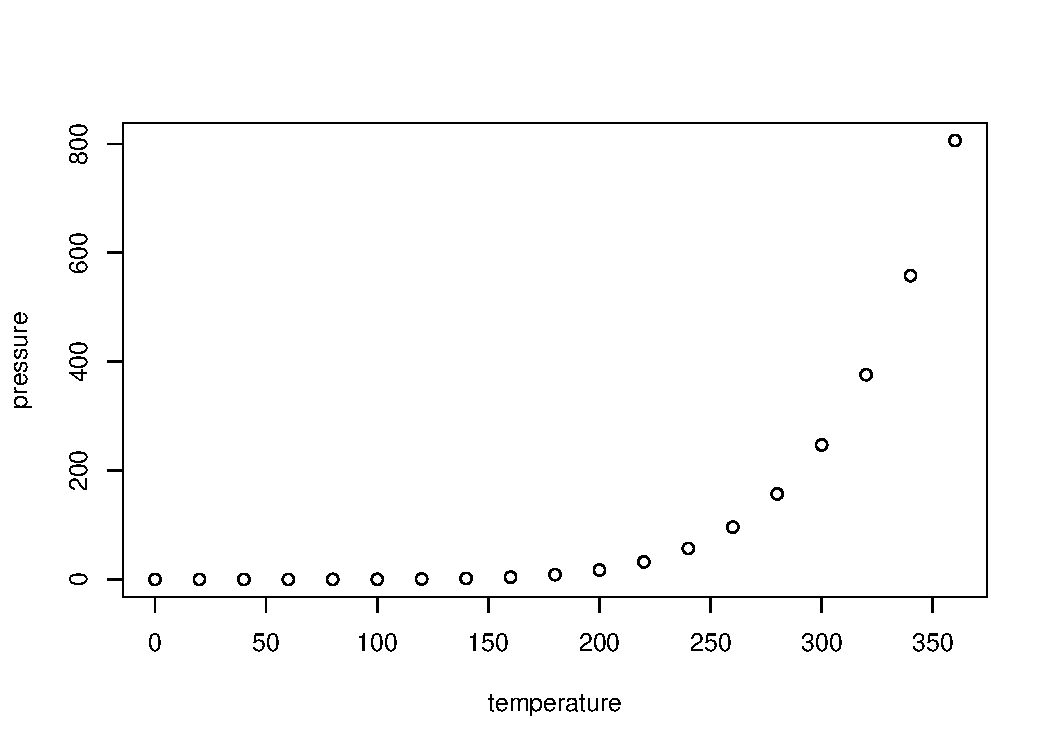
\includegraphics{Guideline-Book_files/figure-latex/pressure-1.pdf}

Note that the \texttt{echo\ =\ FALSE} parameter was added to the code
chunk to prevent printing of the R code that generated the plot.

\newpage

\section{Git / GitHub}\label{git-github}

\textbf{Git} Terminology Features and Advantages of Git TerminologyGit
is a free, open-source \textbf{version control system (VCS)} that helps
manage source code and its development history. It's the most widely
used VCS in the world

\textbf{GitHub} is a website that helps developers store, manage, and
collaborate on software projects.It's a social network for programmers
that encourages collaboration and sharing of code . Github is an online
platform that allows you to store remote repositories of your projects
(Interactable)

\subsection{SOURCE CONTROL / VERSION
CONTROL}\label{source-control-version-control}

\begin{itemize}
\tightlist
\item
  Some System used for tracking your file progress over time .
\item
  It is usually saved in a series of snapshots and branches, which you
  can move back and forth between.
\item
  Prevent against data loss / damage by Creating backup copies of your
  work.
\end{itemize}

Linux is the major / huge project in github Git is a Source Control
Software . It was created by the same person who created Linux
\textbf{Linus Torvalds}

\subsection{Command Prompt}\label{command-prompt}

Before using git/github we need to have a basic idea about command
prompt . Command prompt is a command line interpreter application
available in most Windows operating systems. It's used to execute
entered commands. Most of those commands automate tasks via scripts and
batch files, perform advanced administrative functions, and troubleshoot
or solve certain kinds of Windows issues.

Some of the basic commands prompt codes are :

\begin{Shaded}
\begin{Highlighting}[]
\NormalTok{E}\SpecialCharTok{:} \OtherTok{{-}\textgreater{}}\NormalTok{ To change the drive to E}
\NormalTok{cd }\OtherTok{{-}\textgreater{}}\NormalTok{ To change the directory}

\CommentTok{\# some time we have space in the directory name so we need to use double quotes}
\NormalTok{cd }\StringTok{"C:\textbackslash{}Users\textbackslash{}Deepaneesh R V\textbackslash{}Documents"} \OtherTok{{-}\textgreater{}}\NormalTok{ To change the directory to Documents}
\NormalTok{cd.. }\OtherTok{{-}\textgreater{}}\NormalTok{ To go back to the previous directory}
\NormalTok{cd}\SpecialCharTok{/} \OtherTok{{-}\textgreater{}}\NormalTok{ To go to the root }\FunctionTok{directory}\NormalTok{(Home)}
\NormalTok{cd}\SpecialCharTok{/}\NormalTok{mnt}\SpecialCharTok{/}\NormalTok{E }\OtherTok{{-}\textgreater{}}\NormalTok{ To change the directory to E drive }
\NormalTok{dir }\OtherTok{{-}\textgreater{}}\NormalTok{To list the files }\ControlFlowTok{in}\NormalTok{ the directory}
\NormalTok{mkdir }\OtherTok{{-}\textgreater{}}\NormalTok{ To create a new directory}
\NormalTok{rmdir }\OtherTok{{-}\textgreater{}}\NormalTok{ To remove a directory}
\end{Highlighting}
\end{Shaded}


\end{document}
